\subsection{Opgave 34}

Figuren viser graferne for to eksponentialfunktioner f og g bestemt ved

\begin{align*}
    f(x) = 0,5^x \\
    g(x) = 1,5^x
\end{align*}

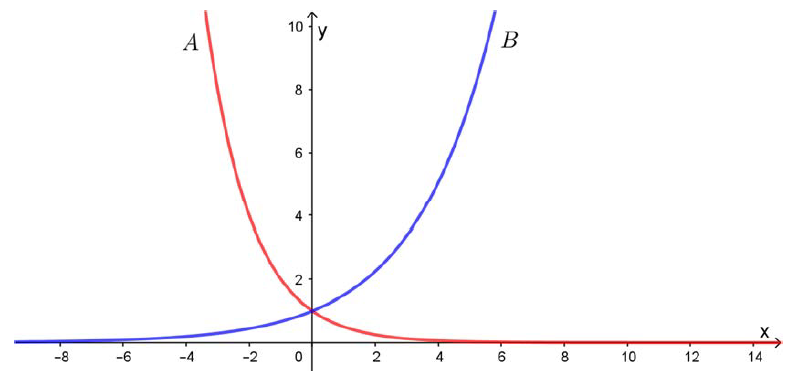
\includegraphics[width=8cm]{Opgave_31-40/Opgave_34/34.png}

Afgør hvilken graf, der hører til hvilken funktion.

\ans

Vi ved at eksponentialfunktioner har den generelle forskrift

$f(x) = a^x$

Vi ved yderligere at for en eksponentialfunktion gælder det at 

\begin{align*}
    &\text{funktionen er aftagende når} \hspace*{2mm} 0 < a < 1\\
    &\text{funktionen er voksende når} \hspace*{3mm} a > 1
\end{align*}

Da funktionen $f(x)$ har a værdien $a = 0,5$ ved vi at den er aftagende og derfor svarer til den røde funktion A som er aftagende.

Da funktionen $g(x)$ har a værdien $a = 1,5$ ved vi at den er voksende og derfor svarer til den blå funktion B som er voksende.
